\documentclass[10pt,a4paper]{article}
\usepackage[utf8]{inputenc}
\usepackage[english]{babel}
\usepackage{graphicx}
\usepackage{lmodern}
\usepackage{kpfonts}
\usepackage{subcaption}
\usepackage{dsfont}
\usepackage{wrapfig}
\usepackage[left=2cm,right=2cm,top=2cm,bottom=2cm]{geometry}
\author{Megi Dervishi}
\title{Machine Learning Homework}
\begin{document}
\maketitle
\subsection*{Exercise 1}
The dataset is seperated into two: train and test. The nonMNIST dataset is composed by images $X_i$ which are 28 by 28 pixels ranging from 0 to 255. I have normalized them. Hence the input space is $\mathcal{X} \in [0,1]^{784}$ and $\mathcal{Y} \in \{1,-1\}$ i.e. the image will have a label  $Y_i = 1$ if it shows A and -1 otherwise as seen in the Figure 1. The training set is then $D := \{(X_i, Y_i), i = 1, \cdots , n\}$ where $n = 6000$. The training images are reshaped into a matrix of 6000 by 784 and the matrix for the testing images is 750 by 784.  Whereas the vector for training labels is $6000$ by $1$ and testing labels is $750$ by 1. An image is a vector of $784$ by $1$.  The total amount of "A"s in the training dataset is 2000 and in the testing is 250. 
\begin{figure}[h!]
\centering
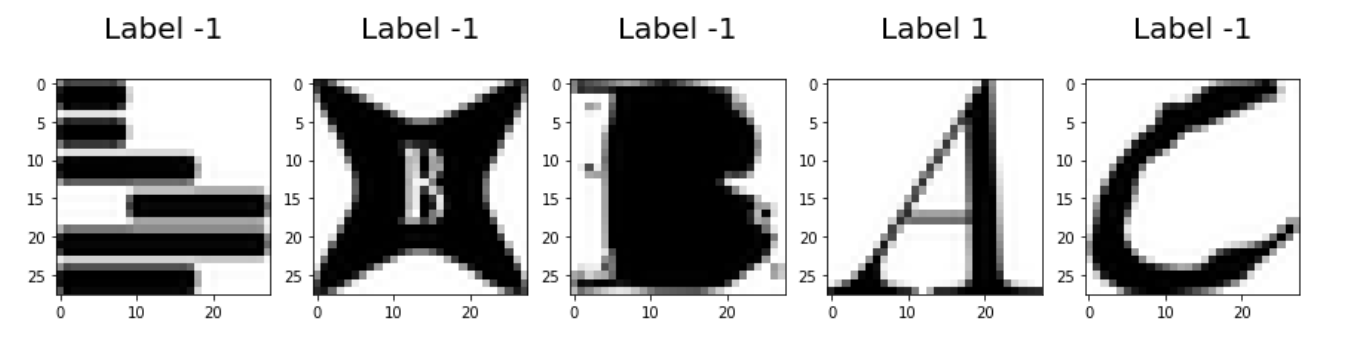
\includegraphics[width = 0.4\textwidth]{figures/img1}
\caption{Examples from the data set}
\end{figure}
\subsection*{Exercise 2}
\textbf{(a)} 
We denote by $D := \{(X_i, Y_i), i = 1, \cdots , n\}$  the training dataset where $n = 6000$. We make an assumption that $(X_i,Y_i)$ are realization i.i.d. random variables from a distribution $v$. The empirical risk for the 0-1 loss (left) and the true risk (right) are as follows:
$$
\hat{R}_n(f) = \frac{1}{n}\sum^n_{i=1} \mathds{1}_{f(X_i) \neq Y_i} \quad \quad  R(f):= \mathbb{E}[\mathds{1}_{f(X)\neq Y}\, | \, D] \quad \text{where } \quad (X,Y) \sim v$$
The empirical risk using the 0-1 loss is not a convex function and not continuous hence the usual methods of minimization using its gradient are not applied because if a function is not convex then you are not guaranteed to reach a minimum and if it is discontinuous then the gradient can be ill-defined. Furthermore if we were to brute force in order to find the minimum, this is an exponential computation which makes it complicated. \\\\
\textbf{(b)} We use the test data to check if the estimator overfits or underfits the training data. The estimator is found by training the learning model using the train data. It is important that the train data and the test data are from the same distribution $v$ but are not the same. Otherwise we would be unable to assess if the learning model has overfitted/underfitted or not i.e we cannot asses whether we have a good estimator. \\\\
\textbf{(c) }\textbf{ Linear least square regression} (LLS). Let $\ell_2(f(X_i), Y_i)$ be the square loss function  and $f:\mathcal{X} \rightarrow \mathcal{Y}$ be an estimator. Also let $n = 6000$ and $d = 784$. The LLS regression optimization problem aims to minimize the empirical risk  given by: 
$$ \hat{R}_n(f) = \frac{1}{n}\sum_{i=1}^n \ell_2(f(X_i),Y_i ) =  \frac{1}{n}\sum_{i=1}^n (f(X_i) - Y_i )^2$$
In the linear model we have that $f$ can be parametrized by a vector $\theta$ as  $f \in \mathcal{F} := \{x \mapsto \theta^Tx : \theta \in [0,1]^{d} \}$. Thus we get $\hat{R}_n(\theta) = \frac{1}{n}\sum_{i=1}^n (\theta^T X_i - Y_i )^2$ which we can express in matrix notation as follows: 
\begin{align*} \hat{R}_n(\theta) = \frac{1}{n}\sum_{i=1}^n  ||\mathbf{X}\theta - \mathbf{Y}||_2^2  \quad \text{ where } \quad ||\cdot ||_2 \text{ is the } L_2 \text{ norm. }
\end{align*}
To avoid confusion of notation in this report we denote in bold the design matrix $\mathbf{X} \in [0,1]^{n \times d}$ the rows of which are $X_i^T$  and $\mathbf{Y} = (Y_1,\cdots,Y_n)^T \in \{-1,1\}^n$. In the following exercise in order to minimize the risk we compute the closed form formula for the gradient (following below)  and use it to apply gradient descent.
$$\nabla_{\theta} \hat{R_n}= \frac{2}{n}\sum_{i=1}^n X_i(\theta^TX_i - Y_i) = \frac{2}{n} (\mathbf{X}^T\mathbf{X}\theta - \mathbf{X}^T \mathbf{Y})$$\\\\
\textbf{Linear Logistic regression} 
Similarly for LLR we simply replace $\ell_2(f(X_i),Y_i)$ with $\ell_3(f(X_i),Y_i)$, then the LLR optimization problem aims to minimize the empirical risk (left). Using the gradient (right) we apply it to gradient descent in order to minimize the risk:
$$\hat{R}_n(\theta) = \frac{1}{n} \sum ^n_{i=1}\log(1 + e^{-Y_i\theta^TX_i} ) 
\quad \quad \quad 
\nabla_{\theta}\hat{R_n} = \frac{1}{n}\sum_{i=1}^n -X_i Y_i \frac{e^{-Y_i\theta^TX_i}}{1+e^{-Y_i\theta^T X_i} } $$
\subsection*{Exercise 3}
\textbf{a)} We have chosen the following step-sizes and obtain the following results. 

\begin{figure}[h!]
\begin{subfigure}[b]{0.5\textwidth}
\centering
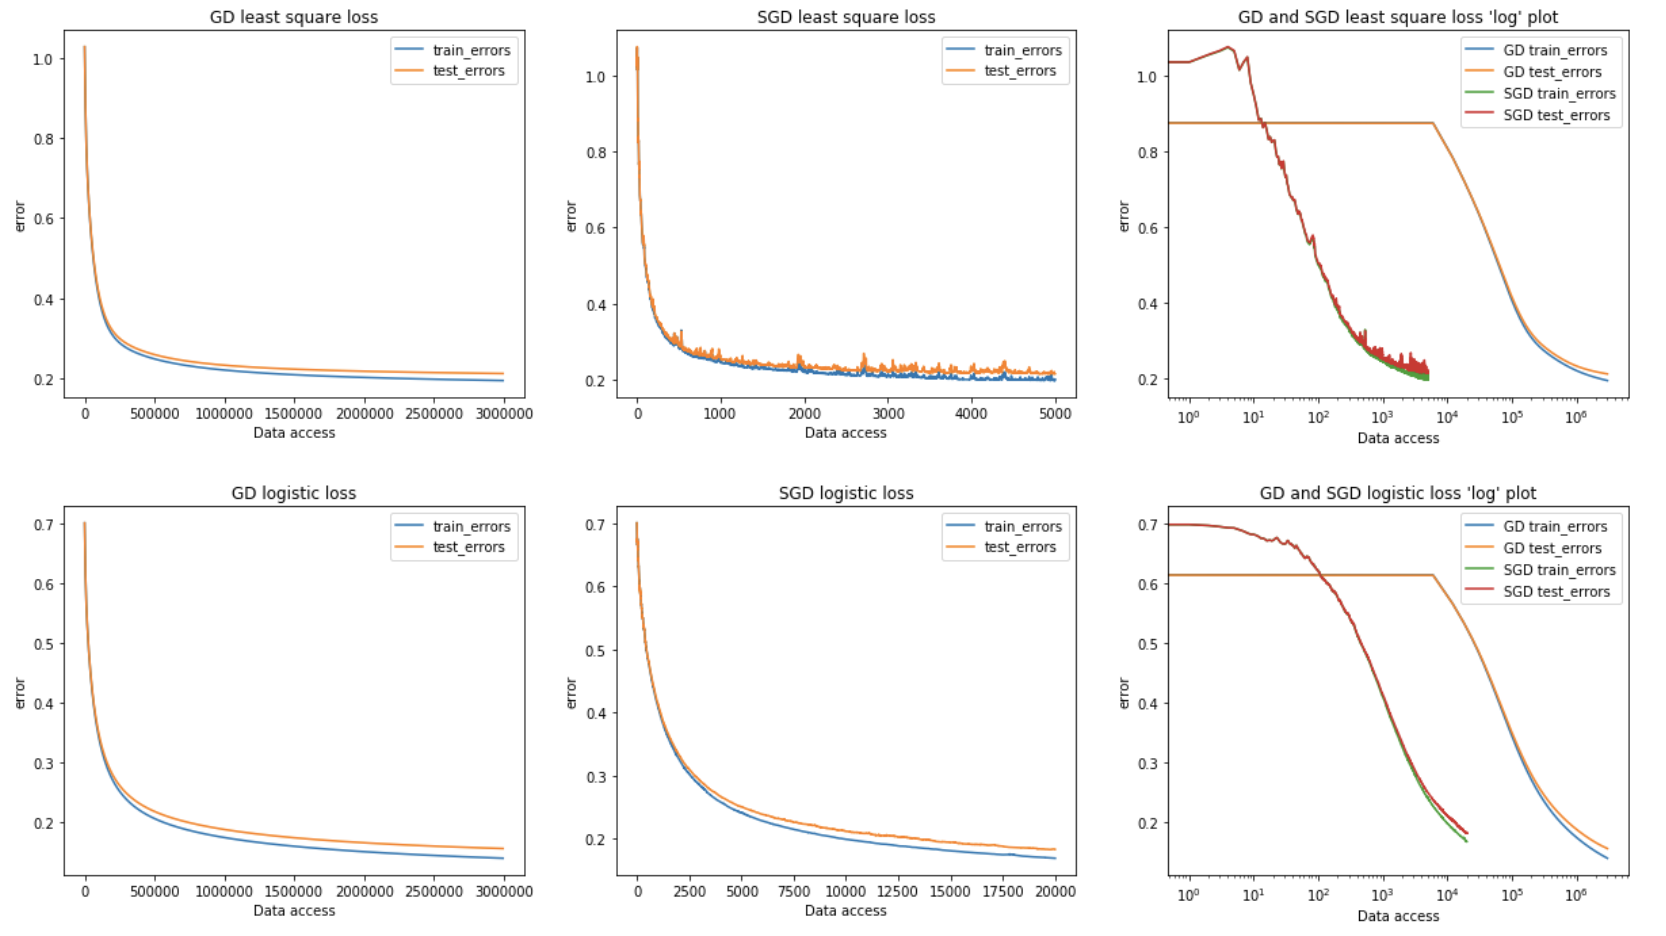
\includegraphics[width = \textwidth]{figures/res}
\caption{Results}
\end{subfigure}
\begin{subfigure}[b]{0.5\textwidth}
\centering
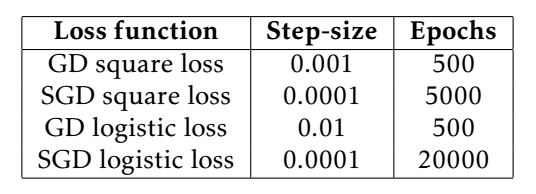
\includegraphics[width = \textwidth]{figures/steps}
\caption{Step-sizes and epochs for each loss function}
\end{subfigure}
\begin{subfigure}[b] {0.5 \textwidth}
\centering
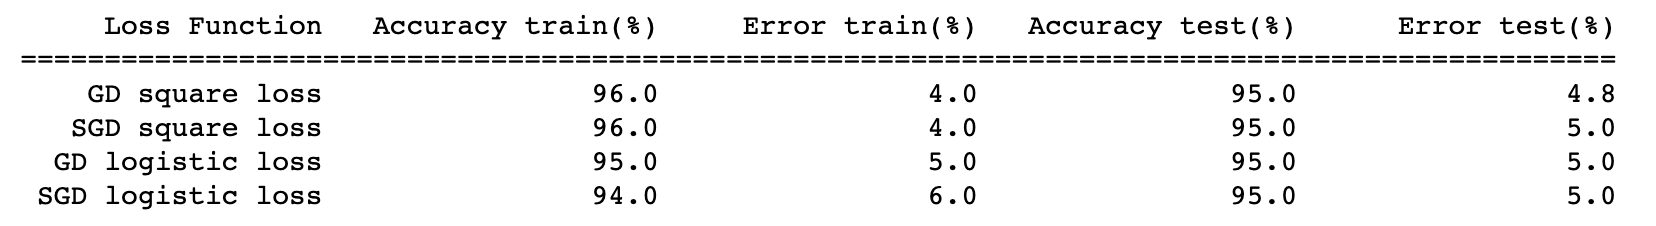
\includegraphics[width = 1.1\textwidth]{figures/acc}
\caption{Accuracy and error}
\end{subfigure}
\end{figure}



\begin{wrapfigure}{r}{0.4\textwidth}
\centering
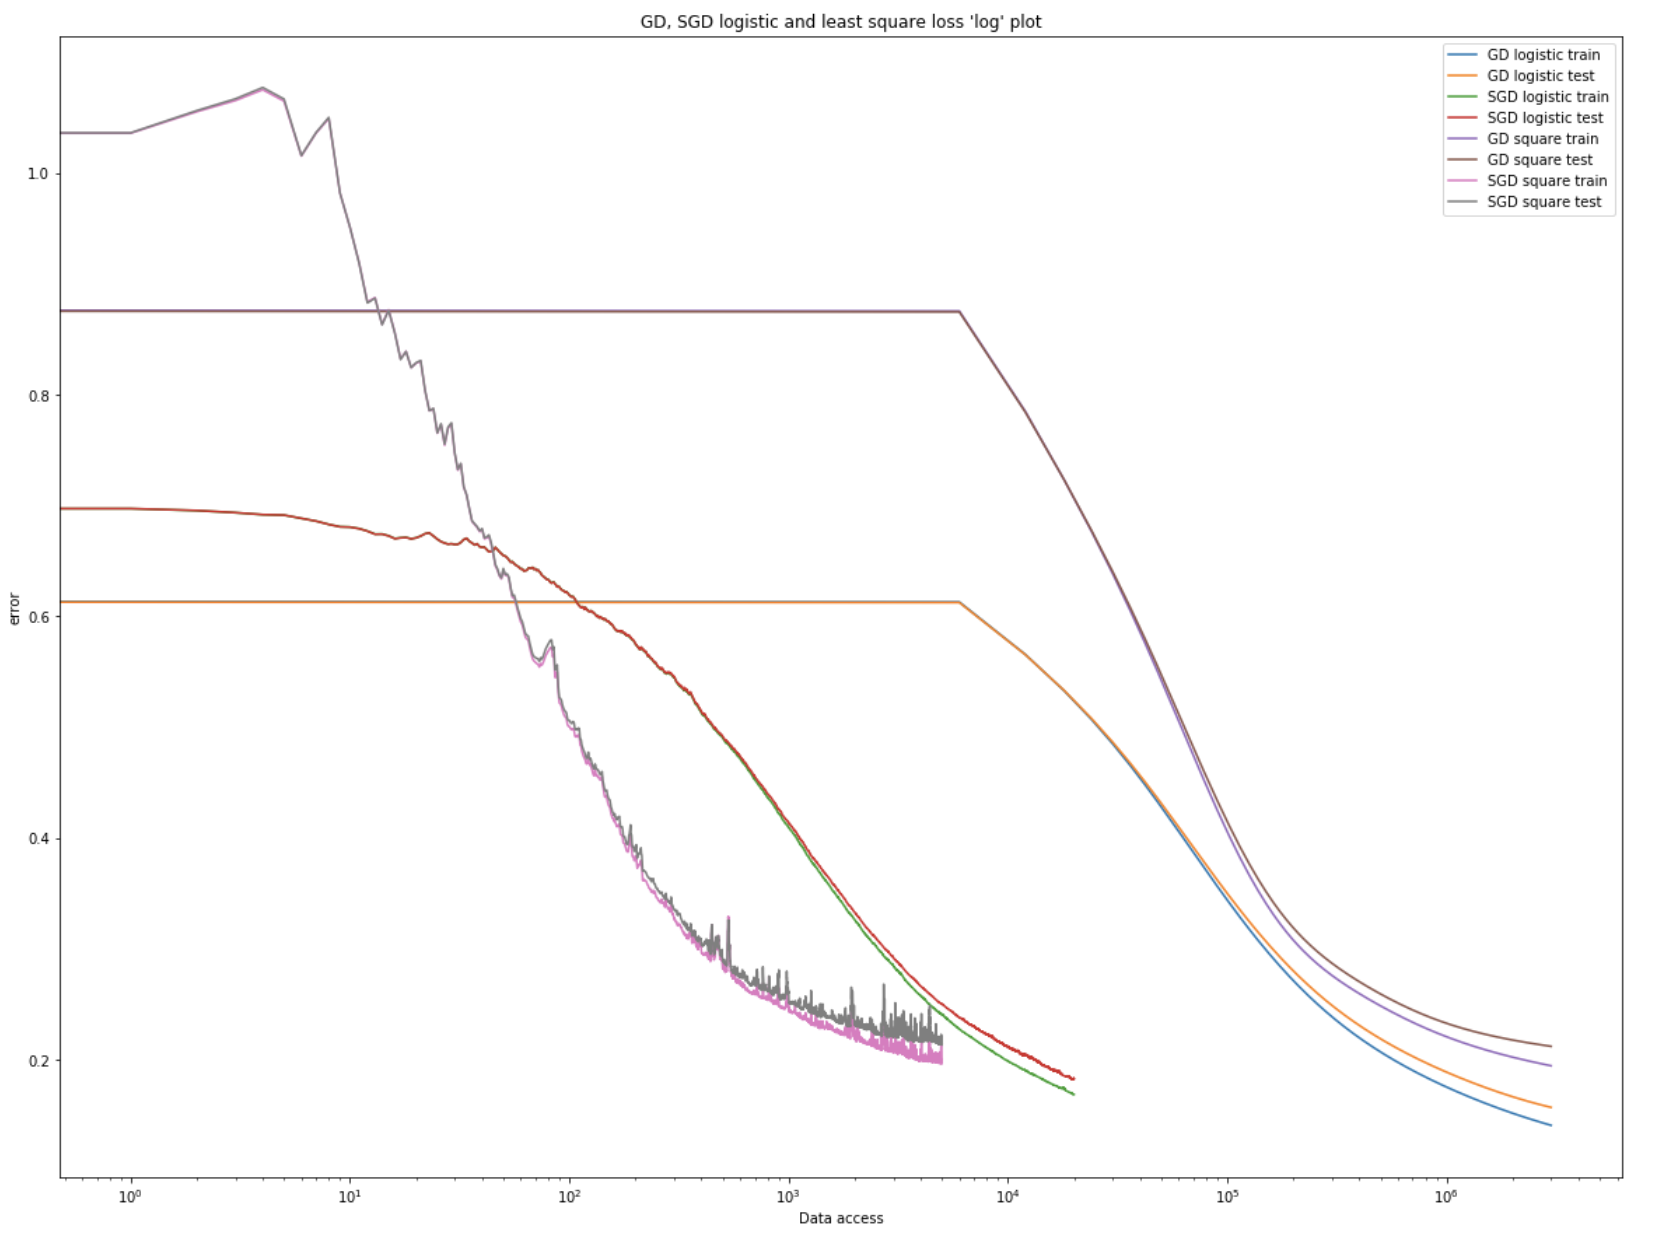
\includegraphics[width = 0.5\textwidth]{figures/graph}
\caption{}
\end{wrapfigure}

The first obvious conclusion we can draw is that the test and train errors are exponentially decreasing in the same manner. We therefore are not over-fitting. Second  we observe in figure 3  that the SGD converges faster in terms of data access compared to GD for both loss functions. From figure 3 we also notice a difference in behavour in between the loss functions which is particularly visible for SGD (red,green,gray and pink curves). The square loss starts decreasing earlier but slower than the logistic loss (approximately twice as slow). Hence we can conclude that for a small amount of data access it's better to use the square loss while for huge data access logistic may be more interesting. Overall the accuracy on the test images for all the methods are around $95\%$ i.e. the found estimator is indeed a good one. This points to the fact that the remaining $5\%$ of the test images can be "hard" to learn by the model or the features of it are under-represented in the training set like the first image from figure 1 . This could be solved with data augmentation. A last improvement could be to not choose the step-size or max\_iterations manually but with a particular algorithm. This could guarantee a better step-size and perhaps increase the accuracy of the new estimator $\theta$. \\\\
\textbf{b)}  The results of the estimator are seen in figure 4 (a). We notice a superposition of an "A" shape with positive values and "C", "B" shape with negative values. This is good because the estimator will try to recognize the features of "A" by associating positive numbers to the features of "A" and negative numbers to those of "B" and "C".\\\\
\textbf{c)} As seen in figure 4 (b) with the increase of $t$ we have a better accuracy since the features of "A","B" and "C" are more refined in the estimator. We also notice that the estimator ($t = 10000$) for logistic is "sharper" (more contrast on the features) than the estimator of the square loss.
\begin{figure}[h!]
\begin{subfigure}[b] {0.5 \textwidth}
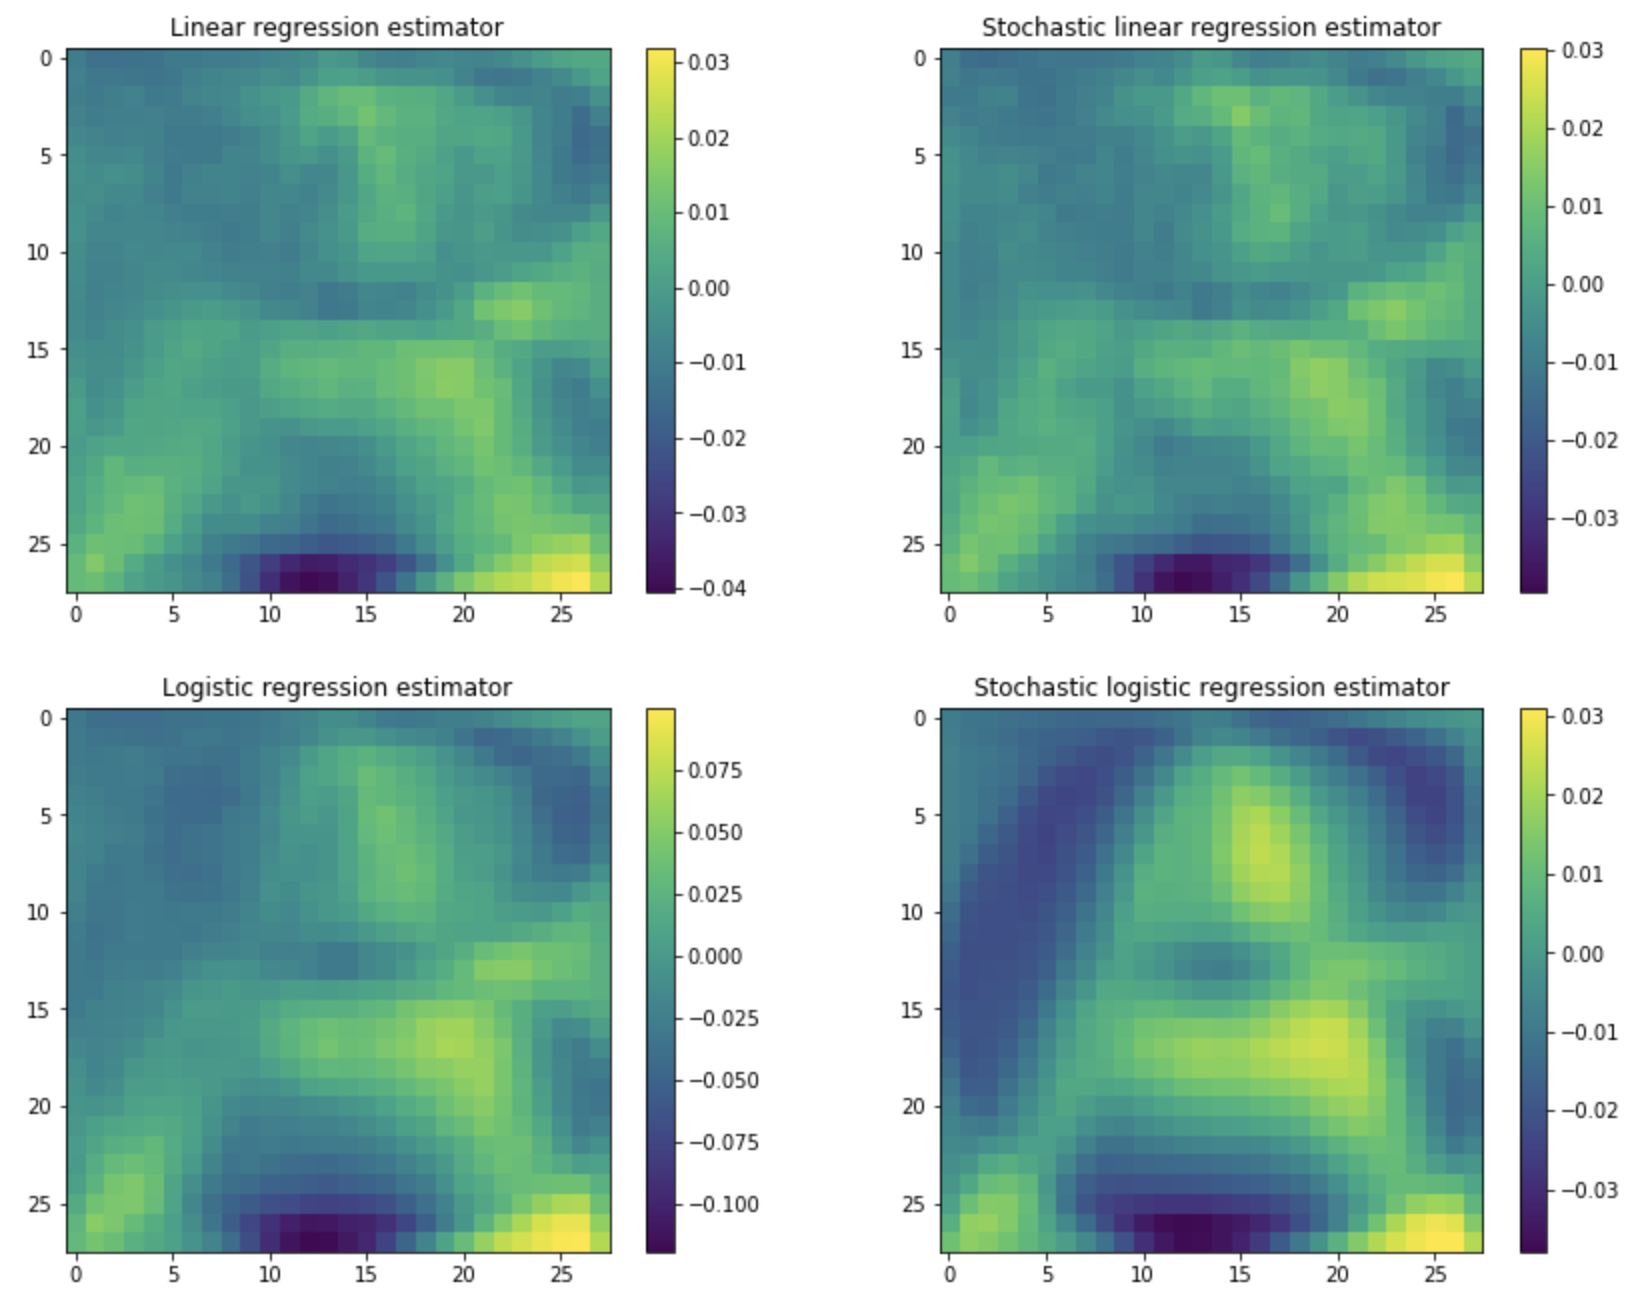
\includegraphics[width = \textwidth]{figures/theta}
\centering
\caption{The estimators for SGD square and logistic loss}
\end{subfigure}
\begin{subfigure}[b]{0.5 \textwidth}
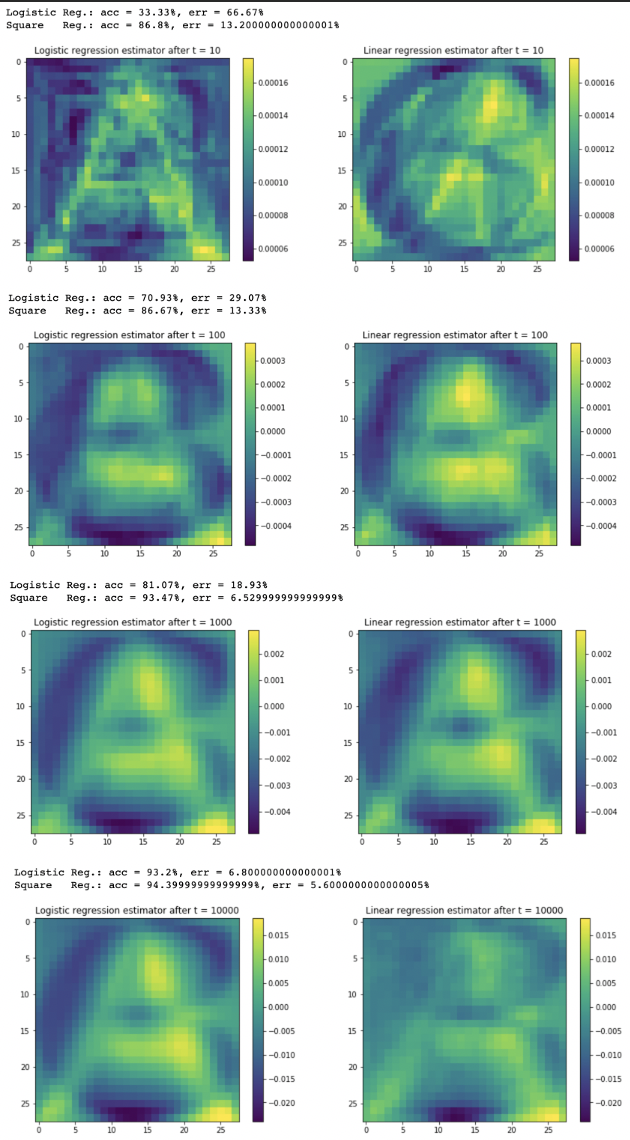
\includegraphics[width = 0.5\textwidth]{figures/t}
\centering
\caption{The estimators for SGD square and logistic loss}
\end{subfigure}
\caption{}
\end{figure}


\subsection*{Exercise 4}
\textbf{a)} KNN works as follows. We take an unlabeled data.  We compute the distance between that data and every other training data using in our case the $\ell_2$ metric i.e. euclidean distance. Then from the possible distances we takes the k smallest ones i.e k neareast neighbours (as the name suggests) and classify the unlabeled data in the category that is the most represented by the neighbours.\\\\ 
\textbf{b)} 
Obviously for $k = 1$ we have 0 error on the training set as you always choose yourself "correctly". Then as k increases the train error increases whereas the test error is somewhat constant. As the footnote suggest we can not say much from this graph. One interesting idea is to use dimensionality reduction such as PCA or t-SNE before running KNN to see if we can improve the predictive performance.\\
\textbf{c)}
\begin{figure}[h!]
\begin{subfigure}[b]{0.5\textwidth}
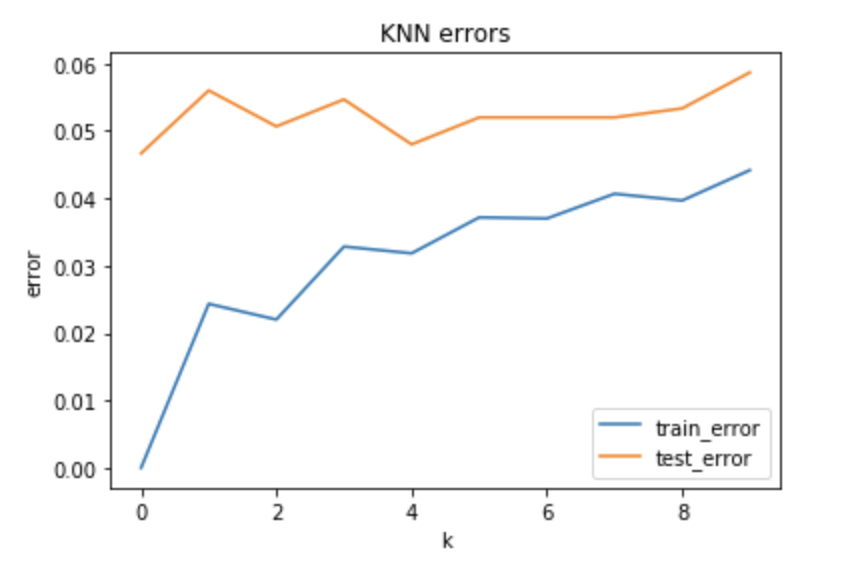
\includegraphics[width =  0.7 \textwidth]{figures/knn}
\centering
\caption{KNN errors}
\end{subfigure}
\begin{subfigure}[b] {0.5 \textwidth}
\centering
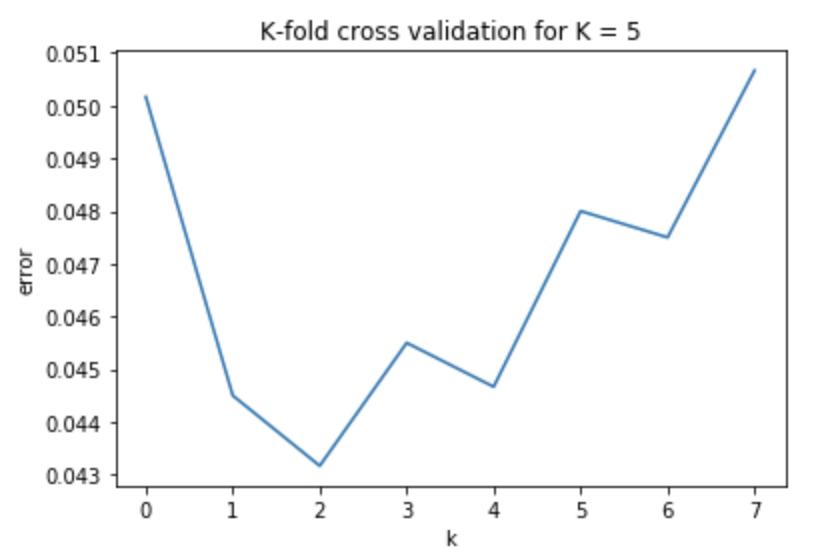
\includegraphics[width = 0.7 \textwidth]{figures/cross}
\caption{K - fold Cross validation  for K = 5 for Exercise 4 c  }
\end{subfigure}
\end{figure}

\subsection*{Exercise 5}
\begin{center}
\begin{tabular}{| c | c | c| c| }
\hline
 & Logistic & Linear & K-NN  (K=8)\\
 \hline
Empirical & 0.05 & 0.04 & 0.04\\
\hline
Test error & 0.05 & 0.05 & 0.06\\
\hline
\end{tabular}
\end{center}


\end{document}